\documentclass[aspectratio=169,11pt]{beamer}

\usepackage[T1]{fontenc}
\usepackage{libertine}
\usepackage[scaled=0.85]{inconsolata}
\usepackage{booktabs}
\usepackage{listings}
\usepackage{xcolor}
\usepackage{tikz}
\usetikzlibrary{arrows.meta, positioning}

%% Palette validated for the figures (light mode; CVD protan dE 9.4, above floor).
\definecolor{pine}{HTML}{1C9970}
\definecolor{pinedark}{HTML}{135C44}
\definecolor{amber}{HTML}{C4761A}
\definecolor{ink}{HTML}{1D2321}
\definecolor{muted}{HTML}{5C6663}
\definecolor{rulegrey}{HTML}{DFE3DE}
\definecolor{paper}{HTML}{FBFBF9}

\usetheme{default}
\usecolortheme{default}
\setbeamercolor{background canvas}{bg=paper}
\setbeamercolor{normal text}{fg=ink}
\setbeamercolor{frametitle}{fg=pinedark}
\setbeamercolor{structure}{fg=pine}
\setbeamerfont{frametitle}{size=\large, series=\bfseries}
\setbeamertemplate{navigation symbols}{}
\setbeamertemplate{itemize items}[circle]
\setbeamertemplate{footline}{%
  \hfill\usebeamerfont{footline}\color{muted}\scriptsize
  \insertframenumber\hspace{2.2em}\vspace{1.1em}}

\lstset{
  basicstyle=\ttfamily\scriptsize\color{ink},
  commentstyle=\color{muted}\itshape,
  keywordstyle=\color{pinedark}\bfseries,
  morekeywords={not},
  breaklines=true, columns=fullflexible,
  frame=leftline, rulecolor=\color{pine}, xleftmargin=8pt, framexleftmargin=4pt,
  literate={<-}{{$\,\leftarrow\,$}}3 {->}{{$\,\rightarrow\,$}}3,
}

\newcommand{\bignum}[2]{%
  \begin{center}
    {\fontsize{54}{58}\selectfont\color{pine}\texttt{#1}}\\[.5em]
    {\color{muted}\small #2}
  \end{center}}

\begin{document}

{\setbeamertemplate{footline}{}
\begin{frame}[plain]
  \vfill
  {\fontsize{34}{38}\selectfont\color{pinedark}\textbf{Approve once.}}\\[1em]
  {\large\color{ink} A governed logic database for\\
   agentic decision support.}\\[1.2em]
  {\color{muted} Deterministic, explainable inference --- and human approval
  that attaches\\ to the logic rather than to each decision.}\\[2em]
  {\color{muted}\small Group 3 --- Human-Centred, Agentic, Decision-Support AI\\
   Working prototype $\cdot$ 285 tests $\cdot$ three domains}
  \vfill
\end{frame}}

\begin{frame}{The remedy everyone reaches for}
  \vspace{.6em}
  \begin{center}{\Large ``Put a human in the loop.''}\end{center}
  \vspace{1.2em}
  \begin{itemize}
    \setlength\itemsep{.9em}
    \item EU AI Act Article~14 requires effective human oversight of high-risk
      systems.
    \item In practice this means a reviewer approves or rejects
      \textbf{individual decisions}.
  \end{itemize}
  \vspace{1.2em}
  \pause
  \begin{center}\color{amber}\large That unit is the problem.\end{center}
\end{frame}

\begin{frame}{Two structural failures}
  \vspace{.8em}
  \begin{columns}[T]
    \begin{column}{.47\textwidth}
      \textbf{\color{pinedark}It doesn't scale.}\\[.5em]
      {\color{muted}Cost is flat at one review per decision, however large the
      caseload grows.}
    \end{column}
    \begin{column}{.47\textwidth}
      \textbf{\color{pinedark}It becomes ceremony.}\\[.5em]
      {\color{muted}Where the reviewer cannot verify the output, a signature
      transfers blame without improving the decision.}
    \end{column}
  \end{columns}
  \vspace{2em}
  \begin{center}
    The failure is not of oversight.\\[.3em]
    {\large It is a failure of \textbf{\color{pine}unit}.}
  \end{center}
\end{frame}

\begin{frame}{The move}
  \vspace{1.4em}
  \begin{center}\Large
    Take the decision logic \textbf{out of the model}\\[.4em]
    and put it in an \textbf{inspectable database}.\\[1.4em]
    \pause
    Then review \textbf{\color{pine}rules}, not decisions.
  \end{center}
  \vspace{1.6em}
  \pause
  \begin{center}\color{muted}
    A rule reviewed once governs every future case its body matches.\\
    The work amortises instead of repeating.
  \end{center}
\end{frame}

\begin{frame}{Two contributions, and the order matters}
  \vspace{1.2em}
  \begin{columns}[T]
    \begin{column}{.46\textwidth}
      {\color{pinedark}\textbf{1. The logic database}}\\[.5em]
      {\color{muted}Deterministic inference, three-valued evidence, exact bounds
      under missing facts, and a proof you can read.}
    \end{column}
    \begin{column}{.46\textwidth}
      {\color{pinedark}\textbf{2. Governance over it}}\\[.5em]
      {\color{muted}The agent proposes, the engine infers, and approval attaches
      to rules rather than decisions.}
    \end{column}
  \end{columns}
  \vspace{2em}
  \pause
  \begin{center}
    Approving a rule is a promise about \emph{every future case}.\\[.5em]
    {\large That promise is redeemable only if the engine\\
    makes it \textbf{\color{pine}deterministic} and \textbf{\color{pine}legible}.}
  \end{center}
\end{frame}

\begin{frame}{Determinism is not a nice-to-have here}
  \vspace{1em}
  \begin{itemize}
    \setlength\itemsep{.8em}
    \item Terminating fixpoint --- no function symbols, so the derivable set is
      finite. \textbf{Structural, not a timeout.}
    \item Each round matches a snapshot, so a rule's result cannot depend on
      \emph{where in the round it ran}.
    \item Stratification re-checked on \textbf{every insertion} --- because
      rules arrive from an agent over time.
  \end{itemize}
  \vspace{1.4em}
  \pause
  \begin{center}\color{muted}
    A recursive rule the agent proposes cannot hang the system.\\
    Insertion order cannot change the answer.
  \end{center}
\end{frame}

\begin{frame}{``Why not just use a SAT solver?''}
  \vspace{.6em}
  \begin{columns}[T]
    \begin{column}{.48\textwidth}
      \textbf{\color{pinedark}To decide a case --- no}
      \begin{itemize}
        \setlength\itemsep{.55em}
        \item Returns \emph{a} model, not \emph{the} answer --- the choice
          falls to search order, not to policy
        \item A model is not a derivation; the explanation would be
          reconstructed \emph{afterwards}
        \item \textsc{np}-complete; the fixpoint is polynomial and terminates
          structurally
      \end{itemize}
    \end{column}
    \begin{column}{.48\textwidth}
      \textbf{\color{amber}To check the rule base --- yes}
      \begin{itemize}
        \setlength\itemsep{.55em}
        \item Contradiction: any input deriving \emph{both} outcomes?
        \item Subsumption: already implied by an approved rule?
        \item Dead rule: can this body ever fire?
      \end{itemize}
      \vspace{.4em}
      {\small\color{muted} Existential questions over all inputs --- exactly
      the shape a solver is for.}
    \end{column}
  \end{columns}
  \vspace{1.2em}
  \pause
  \begin{center}\color{muted}
    Approval is a promise about what a rule will do.\\
    A search-order-dependent answer cannot keep it.
  \end{center}
\end{frame}

\begin{frame}{We do not need one yet --- and that is measurable}
  \vspace{.3em}
  All predicates have arity one, so grounding leaves a propositional problem.
  One engine evaluation: \textbf{0.137\,ms}.
  \vspace{.5em}
  \begin{center}
  \begin{tabular}{lrr}
    \toprule
    \textbf{Pack} & \textbf{Inputs} & \textbf{Exhaustive check} \\
    \midrule
    recruitment          & $2^{10}$ & 0.1\,s \\
    benefits eligibility & $2^{10}$ & 0.1\,s \\
    consumer credit      & $2^{19}$ & 72\,s \\
    \bottomrule
  \end{tabular}
  \end{center}
  \vspace{.6em}
  \pause
  \begin{itemize}
    \setlength\itemsep{.45em}
    \item Enumeration \textbf{cannot disagree with production} --- it \emph{is}
      production. No encoding to get wrong.
    \item Past $\sim$25 observables, or any arity-2 predicate, a solver becomes
      necessary.
    \item The trap: a solver reads $h \leftarrow b$ as material implication;
      stratified semantics takes the \emph{minimal} model. Naive encodings
      report contradictions that cannot occur.
  \end{itemize}
\end{frame}

\begin{frame}[fragile]{The defect we shipped twice}
  \vspace{.8em}
  Standard stratified Datalog closes the world: a fact nobody recorded is
  \emph{false}.
  \vspace{1em}
\begin{lstlisting}
% guarantor(A) is UNKNOWN -- nobody recorded it
mitigated(A) <- guarantor(A).
decline(A)   <- high_risk(A), not mitigated(A).
\end{lstlisting}
  \vspace{.3em}
  \begin{itemize}
    \setlength\itemsep{.5em}
    \item \texttt{mitigated} is blocked by a missing fact $\Rightarrow$ reads as
      \textbf{false}
    \item so \texttt{not mitigated} \emph{succeeds}
    \item and the applicant is declined on a guarantor \textbf{nobody ever
      asked about}
  \end{itemize}
  \vspace{1em}
  \pause
  \begin{center}\color{pinedark}
    Uncertainty has to survive negation, or three-valued evidence\\
    buys you nothing past the first \texttt{not}.
  \end{center}
\end{frame}

\begin{frame}{Exact bounds, in two evaluations instead of $2^k$}
  \vspace{1em}
  With $k$ unknown facts, the honest answer spans every way they could resolve.
  Naively that is $2^{k}$ evaluations.
  \vspace{1.2em}
  \begin{itemize}
    \setlength\itemsep{.65em}
    \item An unknown reachable only \textbf{positively} is minimised at false,
      maximised at true --- set it directly.
    \item Only negatively? Set it the other way.
    \item Only unknowns reachable under \textbf{both} polarities need
      enumerating --- in practice a handful.
  \end{itemize}
  \vspace{1.3em}
  \pause
  \begin{center}\color{pinedark}
    Checked against exhaustive enumeration on random programs \emph{with}
    negation.\\
    {\color{muted}A shortcut nobody compares against the definition is a guess.}
  \end{center}
\end{frame}

\begin{frame}{The engine's claims are tested, not asserted}
  \vspace{.8em}
  \begin{center}
  \begin{tabular}{lr}
    \toprule
    \textbf{Property} & \textbf{Tests} \\
    \midrule
    Bounds exact vs.\ brute-force enumeration   & 55 \\
    Termination and stratification              & 24 \\
    Determinism: same inputs, same answer       & 22 \\
    Proofs: provenance, assumed vs.\ established & 7 \\
    Unknowns survive negation                   & 5 \\
    Value of information                        & 3 \\
    No circular self-support                    & 1 \\
    \midrule
    \textbf{Total} & \textbf{117 of 289} \\
    \bottomrule
  \end{tabular}
  \end{center}
  \vspace{1em}
  \begin{center}\color{muted}\small
    40\% of the suite exists to make approval mean something.
  \end{center}
\end{frame}

\begin{frame}{The result}
  \bignum{36.8}{decisions governed per act of review\\
    16 reviews $\cdot$ 589 decisions $\cdot$ 1{,}000 real credit applications}
  \vspace{.4em}
  \begin{center}\color{muted}\small
    and the ratio is still climbing as the rule base matures
  \end{center}
\end{frame}

\begin{frame}{Oversight cost per decision}
  \begin{center}
    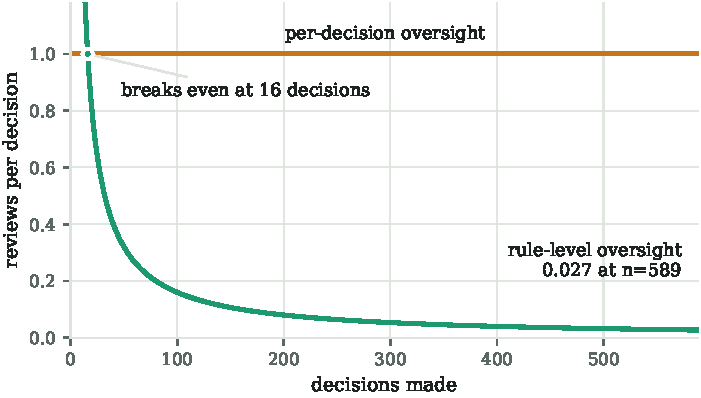
\includegraphics[width=.80\textwidth]{figures/amortisation.pdf}
  \end{center}
  \vspace{-.4em}
  \begin{center}\color{muted}\small
    Reviews are paid up front --- so it is \emph{more} expensive at first,
    and breaks even at 16 decisions.
  \end{center}
\end{frame}

\begin{frame}{The commitment that makes it work}
  \vspace{1.2em}
  \begin{center}
    {\Large The agent \textbf{\color{pine}proposes}.}\\[.5em]
    {\Large Only the engine \textbf{\color{pine}infers}.}
  \end{center}
  \vspace{1.6em}
  \begin{itemize}
    \setlength\itemsep{.7em}
    \item An LLM drafts candidate facts and rules. It never produces a decision.
    \item Inference is a terminating Datalog fixpoint --- same inputs, same
      answer, every time.
    \item Nondeterminism is quarantined \emph{upstream} of a human approval gate.
  \end{itemize}
  \vspace{1em}
  \pause
  \begin{center}\color{muted}
    A hallucinated predicate never becomes a bad decision.\\
    The vocabulary is closed; it becomes a discarded proposal nobody sees.
  \end{center}
\end{frame}

\begin{frame}[fragile]{A rule carries its own governance}
  \vspace{.6em}
\begin{lstlisting}
rule r0003 [p=0.80, origin=mined, status=approved,
            by="reviewer-jd", support=214,
            used=5, right="3/4"]
  high_risk(A) <- overdrawn(A), thin_savings(A).
\end{lstlisting}
  \vspace{.9em}
  \begin{itemize}
    \setlength\itemsep{.55em}
    \item \texttt{used} --- the amortisation count.
    \item \texttt{right} --- a live tally, so strength is \emph{auditable}
      rather than asserted.
  \end{itemize}
  \vspace{.7em}
  \pause
  {\color{muted}Identity is a \textbf{canonical} hash --- variables renumbered,
  body sorted. Otherwise the same rule returns to the queue in different clothes
  and ``approve once'' means nothing.}
\end{frame}

\begin{frame}{Criticality routes review}
  \vspace{.6em}
  \begin{center}
  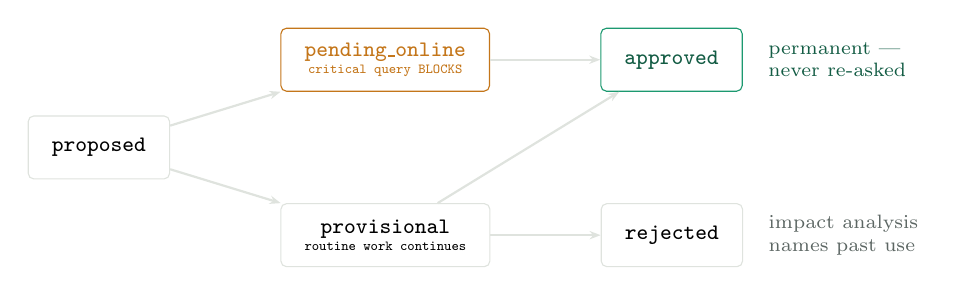
\begin{tikzpicture}[
      box/.style={draw=rulegrey, fill=white, rounded corners=2pt,
                  font=\ttfamily\footnotesize, minimum height=8mm,
                  inner xsep=3mm, align=center},
      hot/.style={box, draw=amber, text=amber},
      ok/.style={box, draw=pine, text=pinedark},
      a/.style={-{Stealth[length=4pt]}, draw=rulegrey, thick}]
    \node[box] (p) {proposed};
    \node[hot, above right=3mm and 14mm of p] (o)
      {pending\_online\\[-1.2mm]{\tiny critical query BLOCKS}};
    \node[box, below right=3mm and 14mm of p] (v)
      {provisional\\[-1.2mm]{\tiny routine work continues}};
    \node[ok, right=14mm of o] (ap) {approved};
    \node[box, right=14mm of v] (rj) {rejected};
    \draw[a] (p) -- (o); \draw[a] (p) -- (v);
    \draw[a] (o) -- (ap); \draw[a] (v) -- (ap); \draw[a] (v) -- (rj);
    \node[right=2mm of ap, font=\scriptsize, text=pinedark, align=left]
      {permanent ---\\never re-asked};
    \node[right=2mm of rj, font=\scriptsize, text=muted, align=left]
      {impact analysis\\names past use};
  \end{tikzpicture}
  \end{center}
  \vspace{.8em}
  \begin{center}
    Criticality attaches to the \textbf{query}.
    Approval attaches to the \textbf{rule}.
  \end{center}
\end{frame}

\begin{frame}[fragile]{The invariant}
  \vspace{1.2em}
  \begin{center}
    {\large A critical decision can only ever be produced by a derivation\\
     in which \textbf{\color{pine}every rule is approved}.}
  \end{center}
  \vspace{1.2em}
\begin{lstlisting}
BLOCKED  critical query q00002 needs approval of: r0001, r0005.
         A critical decision may not rest on unreviewed logic.
\end{lstlisting}
  \vspace{1em}
  \begin{center}\color{muted}
    Enforced in the engine, not by convention --- and re-audited afterwards
    across every decision. \textbf{Zero violations.}
  \end{center}
\end{frame}

\begin{frame}[fragile]{What a decision looks like}
  \vspace{.2em}
\begin{lstlisting}
Answer: P = [0.00, 0.70]
  The interval is 0.70 wide because facts are missing. It is not a
  confidence interval over a model - it spans every way the unknowns
  could resolve.

[rule] app_gap should be declined  p=0.70
  [rule] by r0002: decline(A) <- high_risk(A), not mitigated(A). p=0.88
    (origin document; approved by policy-team; cites s7.1; right 70/191)
    [fact] app_gap is overdrawn      (source: application form, field 3)
  [UNKNOWN] not app_gap has mitigating circumstances
      (ASSUMED, not established)

Missing information, ranked by whether it would change anything:
  app_gap has a guarantor   [DECISIVE]
      if true -> 0.00, if false -> 0.70
\end{lstlisting}
\end{frame}

\begin{frame}{Three things that page does}
  \vspace{1.2em}
  \begin{enumerate}
    \setlength\itemsep{1.1em}
    \item \textbf{Refuses to guess.} A missing fact produces an interval, not a
      number.
    \item \textbf{Names the one question} that would settle it --- and stays
      silent about unknowns that change nothing.
    \item \textbf{Separates assumed from established}, so an interval endpoint
      cannot be misread as a finding.
  \end{enumerate}
  \vspace{1.3em}
  \pause
  \begin{center}\color{muted}
    We shipped (3) wrong twice. \texttt{not mitigated(app)} succeeded because
    nobody had recorded a guarantor ---\\
    and an applicant was declined on an assumption no one had made.
  \end{center}
\end{frame}

\begin{frame}{Does the miner find the right rules?}
  \begin{center}
    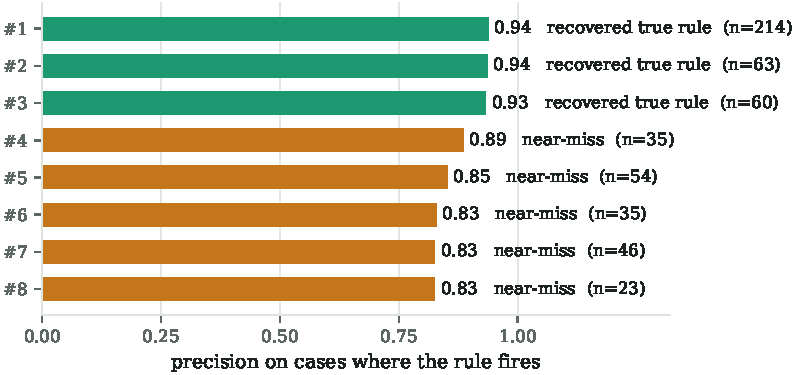
\includegraphics[width=.9\textwidth]{figures/recovery.pdf}
  \end{center}
  \vspace{-.6em}
  \begin{center}\color{muted}\small
    Synthetic domain generated from a rule set that is then withheld ---
    ground truth for \textbf{rules}, not predictions.
  \end{center}
\end{frame}

\begin{frame}{The near-misses are the point}
  \vspace{.9em}
  Two of the five are wrong in ways a reviewer can \emph{check}:
  \vspace{1.1em}
  \begin{itemize}
    \setlength\itemsep{.9em}
    \item One grants eligibility on a \textbf{recent award} --- which policy
      s4.1 says should trigger \emph{referral}.
    \item One reproduces the disability route with the \textbf{capital-limit
      guard dropped} --- it would pay applicants over the savings limit.
  \end{itemize}
  \vspace{1.3em}
  \begin{center}
    Both sit at \textbf{83--85\% precision}. Both look respectable.
  \end{center}
  \vspace{.7em}
  \pause
  \begin{center}\color{pinedark}\large
    That is the case for a human reading rules.
  \end{center}
\end{frame}

\begin{frame}{Then the system found a hole in our own policy}
  \vspace{1em}
  We wrote a lending policy, extracted 8 cited rules --- and it declined to
  decide \textbf{11\% of cases}.
  \vspace{1.2em}
  \begin{itemize}
    \setlength\itemsep{.5em}
    \item \texttt{s7.1} covers elevated risk \emph{without} security
    \item \texttt{s7.2} covers security \emph{without} elevated risk
    \item \textbf{\color{amber}Neither covers an applicant with both.}
  \end{itemize}
  \vspace{1.2em}
  \pause
  \begin{center}
    We wrote it. We hadn't noticed.\\[.5em]
    {\color{muted}A scoring model would have produced a confident number for
    every one of them.}
  \end{center}
\end{frame}

\begin{frame}{We had already built the conventional version}
  \vspace{.9em}
  A hundred simulated screening agents. 8,000 CVs. 1,000 hires.\\
  Each agent may reject a confirmed mismatch or flag a CV for a person.
  \vspace{1.3em}
  \begin{itemize}
    \setlength\itemsep{.8em}
    \item It flags \textbf{5,621 of 8,000} CVs for human review --- 4,012 of them
      cases where the requirements were \emph{met}.
    \item Plus 237 sampled rejection audits.
  \end{itemize}
  \vspace{1.2em}
  \pause
  \begin{center}\color{amber}\large
    5,858 human reviews to make 1,000 hires. 5.9 per hire.
  \end{center}
\end{frame}

\begin{frame}{And it cannot tell you when it is wrong}
  \vspace{1.1em}
  \begin{itemize}
    \setlength\itemsep{.9em}
    \item Its interface says of agent rejections: \emph{``each can be reopened''}.
    \item \textbf{2,142 of 2,379 rejections (90\%) are never shown to anyone.}
    \item Rejections are correct \emph{by construction} --- there is no notion of
      a suitable applicant wrongly rejected.
  \end{itemize}
  \vspace{1.4em}
  \pause
  \begin{center}\color{pinedark}
    An auditor has nothing to find.\\
    Contestability is offered, and can never be exercised.
  \end{center}
\end{frame}

\begin{frame}{Same campaign, rules instead of cases}
  \vspace{.7em}
  \begin{center}
  \begin{tabular}{lrr}
    \toprule
    & \textbf{Agent fleet} & \textbf{Rule base} \\
    \midrule
    One-off rule reviews        & ---     & 8 \\
    Human case reviews          & 5,858   & \textbf{2,558} \\
    Decided without a person    & 0       & 5,442 \\
    Screening logic inspectable & no      & yes \\
    Wrong rejections measurable & no      & \textbf{yes} \\
    \bottomrule
  \end{tabular}
  \end{center}
  \vspace{1.1em}
  \pause
  \begin{center}
    Against a withheld suitability label:
    \textbf{\color{amber}26.4\%} of automatic rejections\\
    are of genuinely suitable applicants.
    \vspace{.5em}

    {\color{muted}Not a good number. But a number --- and the audit queue
    now has something to find.}
  \end{center}
\end{frame}

\begin{frame}{A disparity you can only see if you record it}
  \vspace{1em}
  \texttt{age\_band} and \texttt{sex} are recorded in the data and are
  \textbf{not declared predicates} --- so no rule can be written or mined over
  either.
  \vspace{1.2em}
  \begin{center}
  \begin{tabular}{lrr}
    \toprule
    \textbf{age band} & \textbf{n} & \textbf{auto-rejected} \\
    \midrule
    under 25 & 2,713 & 38\% \\
    25--39   & 3,626 & 39\% \\
    40+      & 1,661 & \textbf{28\%} \\
    \bottomrule
  \end{tabular}
  \end{center}
  \vspace{1em}
  \pause
  \begin{center}\color{muted}
    Over-40s are auto-rejected \emph{less} --- an age-correlated timeline signal
    routes them to a human instead.\\
    A disparity toward more human review is still a disparity.
  \end{center}
\end{frame}

\begin{frame}{What we measured}
  \vspace{1em}
  \begin{center}
  \begin{tabular}{lr}
    \toprule
    \textbf{Result} & \textbf{Value} \\
    \midrule
    Tests establishing engine properties & 117 / 289 \\
    Bounds disagreeing with exhaustive enumeration & 0 \\
    Decisions per act of review (credit) & 36.8 \\
    Generating rules recovered exactly & 3 / 3 \\
    Proposals resting on noise attributes & 0 / 8 \\
    Cases on which written policy was silent & 11\% \\
    Human case reviews vs.\ our agent fleet & $-$56\% \\
    Governance invariant violations & 0 \\
    \bottomrule
  \end{tabular}
  \end{center}
  \vspace{1.2em}
  \begin{center}\color{muted}\small
    Every figure produced by scripts in the repository; both charts generated
    from live runs.
  \end{center}
\end{frame}

\begin{frame}{What we have \emph{not} measured}
  \vspace{1.5em}
  \begin{center}
    {\large\color{amber} No human has reviewed a rule in this system.}
  \end{center}
  \vspace{1.3em}
  36.8 is arithmetic over a working prototype --- not evidence that reviewers
  review rules \emph{well}. If they cannot, the argument fails, and nothing here
  would currently tell us.
  \vspace{1.3em}
  \pause
  \begin{center}\color{pinedark}
    The experiment is unusually clean: show reviewers the eight proposals;\\
    measure whether they approve the correct three.
  \end{center}
\end{frame}

\begin{frame}{Honest limitations}
  \vspace{.9em}
  \begin{itemize}
    \setlength\itemsep{.85em}
    \item \textbf{Credit assignment is crude.} Every rule in a derivation is
      marked right or wrong together.
    \item \textbf{Rejection flags but does not reverse.} It names affected
      decisions and stops --- that judgement isn't ours to automate.
    \item \textbf{The accuracy figure is not a benchmark.} It scores an invented
      policy against real data.
    \item \textbf{The head-to-head is not like-for-like.} The baseline is our
      own prototype, and the two partition work differently.
  \end{itemize}
  \vspace{1.3em}
  \begin{center}\color{muted}
    The system detecting that its own policy is poorly fitted\\
    is the machinery working, not a capability claim.
  \end{center}
\end{frame}

{\setbeamertemplate{footline}{}
\begin{frame}[plain]
  \vfill
  \begin{center}
    {\large Datalog evaluation is from 1977. We borrow it unchanged.}\\[1.4em]
    {\fontsize{21}{25}\selectfont\color{pinedark}What we built is an engine a
    reviewer can trust,\\ and oversight that sits on the logic.}\\[1.6em]
    {\color{ink}A reviewer reads one rule and governs every case it matches.\\
    They can do that \emph{because} the engine makes approval binding\\
    and shows them what the rule did.}
  \end{center}
  \vfill
\end{frame}}

\end{document}
